\chapter{Methodology}

This chapter provides a comprehensive explanation of how each of the research questions listed in \autoref{chap:Introduction} will be addressed.  This involves showing how the proposed solution will be designed, how the research planning will be carried out and how development and testing will be done.

\section{Research Approach for Objectives 1 and 2}

The first objective of this dissertation was to study previous research work conducted on the GN platform and RDF.  Consequently, the second objective was focused on understanding the current limitations of the Genenetwork2 SQL database and exploring how the adoption of RDF could potentially address these constraints.  To meet these two objectives, a comprehensive literature review was conducted.

\section{Research Approach for Objectives 3}

In order to accomplish objectives three and four, a self-documenting Domain Specific Language (DSL) will be developed to facilitate the translation of SQL into RDF.  This DSL will be employed to convert SQL tables into RDF representations, subsequently enabling a comprehensive comparison of RDF performance against that of SQL.

The development methodology that will be adopted for this step is the \textit{Rapid Application Development (RAD)} methodology since it prioritizes development and prototype-building over planning.  It emphasizes the end-user involvement, prototyping, reuse and the use of automated tools \citep*{van2008software}.  This gives the researcher the ability to efficiently execute numerous iterations and updates to the software/model without the need to begin each iteration anew.  This yields a significant advantage, as it facilitates the ability to modify the design, augment functionality and iteratively refine the software/model at a high frequency.

\citet*{van2008software} outlines the four fundamental steps of the Rapid Application Development (RAD) methodology as:

\begin{enumerate}
\item \textbf{Requirements Planning:} In contrast to traditional software development models, the RAD methodology begins by obtaining a general understanding of the requirements rather than seeking a comprehensive list of specifications from end users.  The broad nature of the requirements allows for the segmentation of specific requirements at different points throughout the development cycle.

\item \textbf{Prototyping:} At this stage, actual development occurs.  Prototypes are created featuring various functionalities rapidly, deviating from a strict set of requirements.  Typically, these prototypes are hastily constructed to demonstrate key features.  The final software artifact is only developed during the finalization stage, where the consensus on the desired outcome has been reached.

\item \textbf{Construction:}  In this stage, the working model is transformed into a functional system.  Usually, most bugs, issues and modifications are addressed.

\item \textbf{Cutover:} The final stage of RAD involves the final testing of the system before the system is ready to use by end users.  The cutover phase encompasses intensive scale testing, technical documentation, issue tracking, final customizations and possible system simulations.
\end{enumerate}

Figure \ref{fig:rad-lifecycle} shows the aforementioned RAD life-cycle.

\begin{figure}[H]
  \centering
  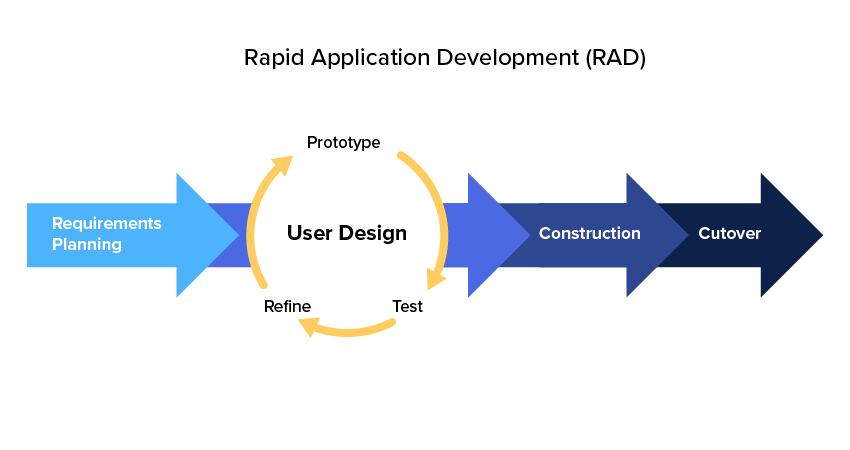
\includegraphics[width=12cm]{RAD}
  \caption{\textit{Rapid Application Development life-cycle}}
  \label{fig:rad-lifecycle}
  \centering
\end{figure}

The following subsections elaborate on the application of the RAD methodology within this dissertation's context.

\subsection{Requirements Planning}

The process of requirements planning is the initial stage in building the DSL.  This stage encompasses activities such as conceptual ideation, during which potential representations of the DSL are brainstormed.  The primary goal is to design a self-documenting DSL that is comprehensible and accessible to human end-users.  Moreover, the DSL should support s-expressions and offer a declarative mapping of SQL query results to a predefined ontology.  Furthermore, in this stage, relevant public and active ontologies will be identified.  The DSL will use these ontologies when transforming data from SQL tables to RDF.

\subsection{Prototyping}

During the prototyping phase, a preliminary version of the DSL will be developed, enabling the exploration of its design and functionality.  This prototype will serve as a proof-of-concept and will be refined based on feedback from stakeholders and potential end-users.  Figure \ref{fig:parser-demo} illustrates the parser's basic operation.

\begin{figure}[H]
\centering
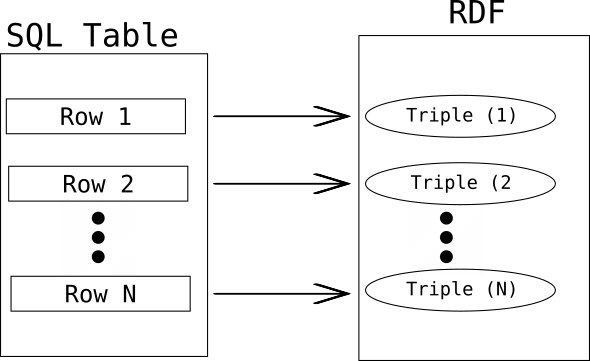
\includegraphics[width=8cm]{parserDemo}
\caption{\textit{The parser operates on each row to produce a valid triple store}}
\label{fig:parser-demo}
\centering
\end{figure}

During the prototyping stage, it is crucial to quickly check whether syntactical errors exist in the RDF output.  To this end, \textit{rapper}, an RDF linter, will be utilized to assess the syntactic correctness of the generated RDF format.  This linting process ensures that the output is free of errors, permitting the data to be ingested into a virtuoso instance.  In the absence of errors detected during the linting procedure, the data can subsequently be uploaded to a running Virtuoso instance.

\subsection{Construction}

The construction phase encompasses the development of a robust, reusable tool.  During this stage, numerous unforeseen challenges, including bugs, issues, and modifications, will be identified and addressed.  In order to prevent regressions, tests will be implemented concurrently with the development process, ensuring the tool's reliability and functionality.

\subsection{Cut-off}

During this final stage, the Domain Specific Language (DSL) will be used to convert GeneNetwork tables into RDF format.  Components of GeneNetwork that rely extensively on metadata will be restructured to utilize RDF.  A comparison between SQL and RDF performance will be assessed.

\section{Validation}

The final objective of this dissertation is to validate this dissertation by comparing the performance of RDF against SQL/flat-files.  To validate the findings in this dissertation, performance benchmarks will be conducted to compare the efficiency of RDF, SQL and flat-files in different scenarios.  The performance benchmarks will include measuring the time required to execute specific queries.  Moreover, functionalities that can be achieved using SPARQL but not SQL will be identified.
